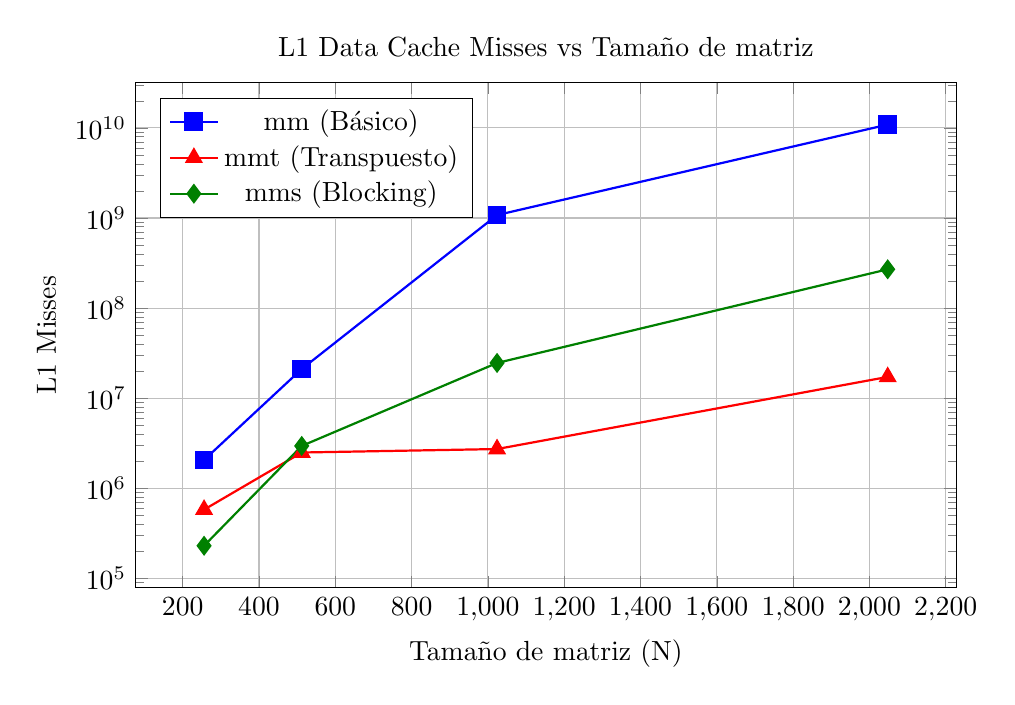
\begin{tikzpicture}
    \begin{axis}[
        title={L1 Data Cache Misses vs Tamaño de matriz},
        xlabel={Tamaño de matriz (N)},
        ylabel={L1 Misses},
        legend pos=north west,
        grid=major,
        width=12cm,
        height=8cm,
        ymode=log,
    ]
        \addplot[
            color=blue,
            mark=square*,
            thick,
            mark size=3pt,
        ]
        coordinates {
            (256, 2065110)
            (512, 21099084)
            (1024, 1078916990)
            (2048, 10888472604)
        };
        \addlegendentry{mm (Básico)}
        \addplot[
            color=red,
            mark=triangle*,
            thick,
            mark size=3pt,
        ]
        coordinates {
            (256, 579849)
            (512, 2496563)
            (1024, 2728198)
            (2048, 17241719)
        };
        \addlegendentry{mmt (Transpuesto)}
        \addplot[
            color=green!50!black,
            mark=diamond*,
            thick,
            mark size=3pt,
        ]
        coordinates {
            (256, 230367)
            (512, 2953415)
            (1024, 24620828)
            (2048, 269646118)
        };
        \addlegendentry{mms (Blocking)}
    \end{axis}
\end{tikzpicture}
